\documentclass{article}[11pt]
\oddsidemargin 0in \evensidemargin 0in \topmargin 0in
\columnsep 10pt \columnseprule 0pt 
\marginparwidth 90pt \marginparsep 11pt \marginparpush 5pt 
\headheight 0pt \headsep 0pt 
%\footheight 0pt \footskip 0pt 
\textheight 9.0in \textwidth 6.5in

\usepackage{graphicx}

\begin{document}

\hspace{2in} Name: (Print) \underline{\mbox{\hspace{3.5in}}}\\

\begin{center}
{\Large STATISTICS 201 - Written Homework Chapter 3}\\[3mm]
\end{center}

\begin{enumerate}

\item Michael Jordan is highly renowned basketball player who played for 15 seasons in the NBA.  The following table contains the average points per game scored by Jordan in each of his 15 seasons.

\begin{center}
\begin{tabular}{|l|c||l|c||l|c|} \hline
Year & Avg Pts/Game & Year & Avg Pts/Game & Year & Avg Pts/Game 
\\ \hline
1984 & 28 & 1989 & 34 & 1995 & 30 \\
1985 & 23 & 1990 & 32 & 1996 & 30 \\
1986 & 37 & 1991 & 30 & 1997 & 29 \\
1987 & 35 & 1992 & 33 & 2001 & 23 \\
1988 & 33 & 1994 & 27 & 2002 & 20 \\ \hline
\end{tabular}
\end{center}

\begin{enumerate}
\item {\em (3 pts)} Make a stem and leaf display of the average number of points per game that Michael Jordan scored per season.  Do this by hand, use a split stem, and ensure that the leaves are sorted numerically. Describe the shape of this distribution. \\

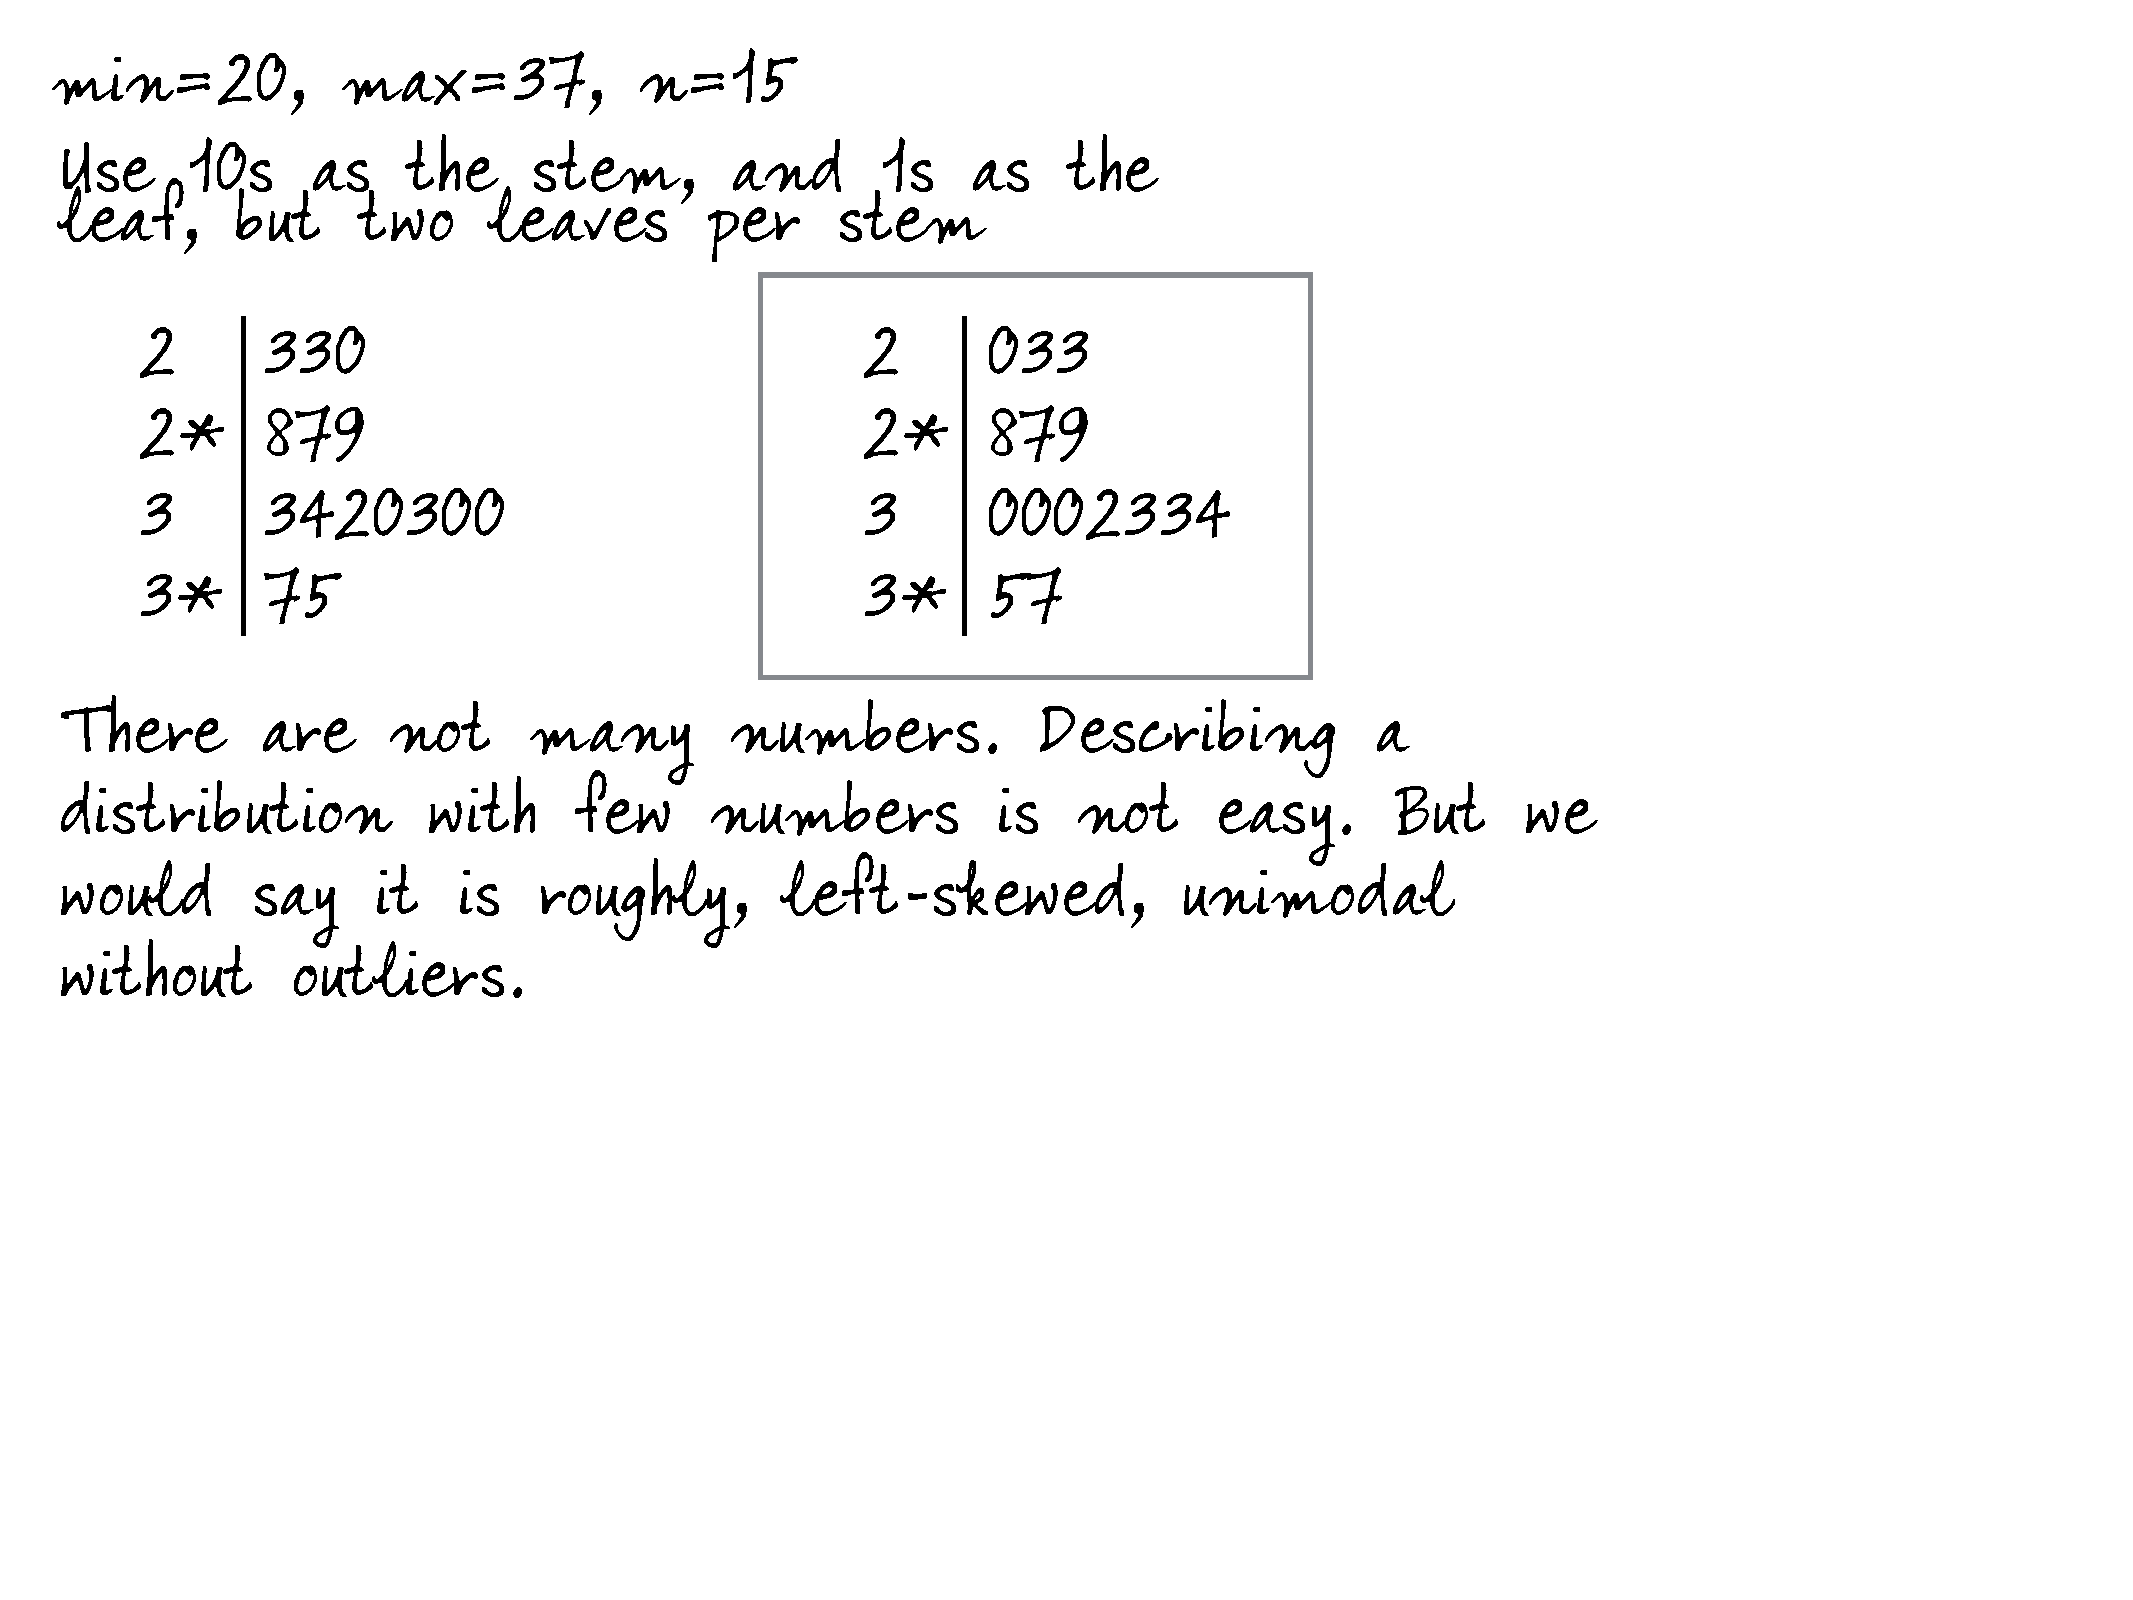
\includegraphics[width=4in]{hwk3-stuff.pdf}

\item  {\em (2 pts)} Make a line plot of average number of points per game by year. Describe the pattern of points relative to time. \\

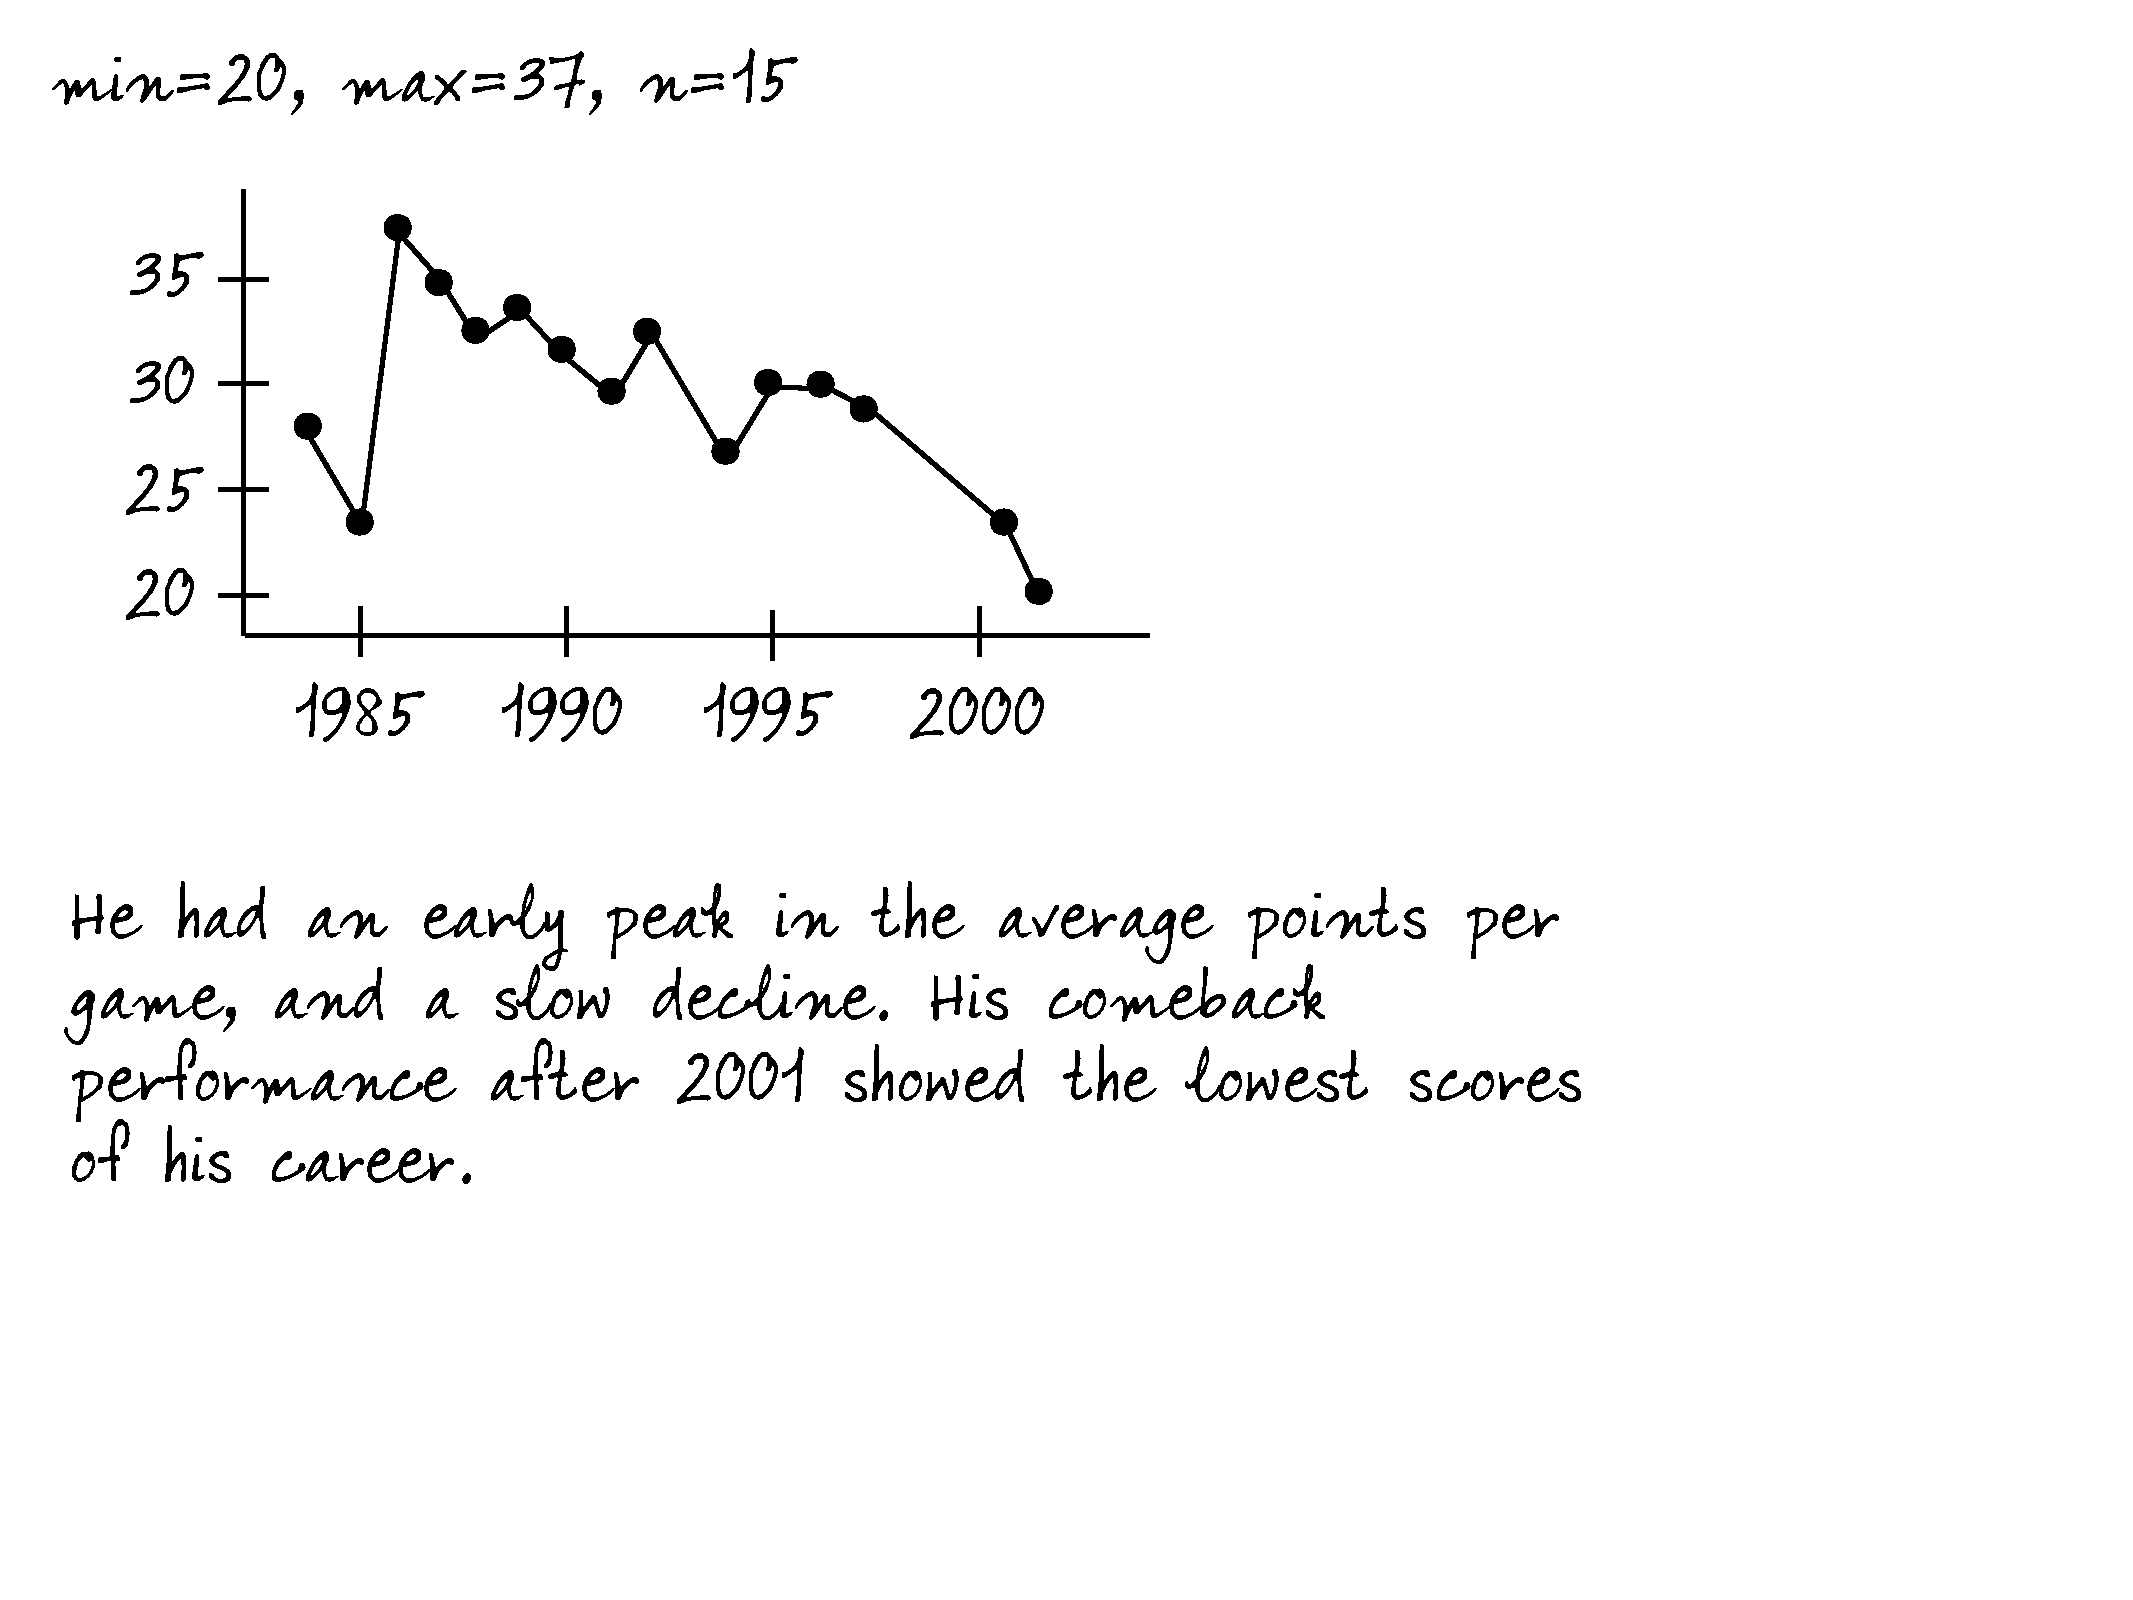
\includegraphics[width=4in]{hwk3-stuff2.pdf}

\end{enumerate}

\newpage
\item For this part of the assignment you will be using data collected on IA high school quarterbacks for the 2012 season.  

\begin{enumerate}
\item {\em (2 pts)} Describe the Who for this data.\\

{\em The IA high school quarterbacks who played in 2012.}

\item {\em (3 pts)} Use intRo to obtain the a histogram of yards thrown (Yards), with a suitable bin width.  Describe the shape of the distribution of this variable. Print out the output and turn it in with this assignment.

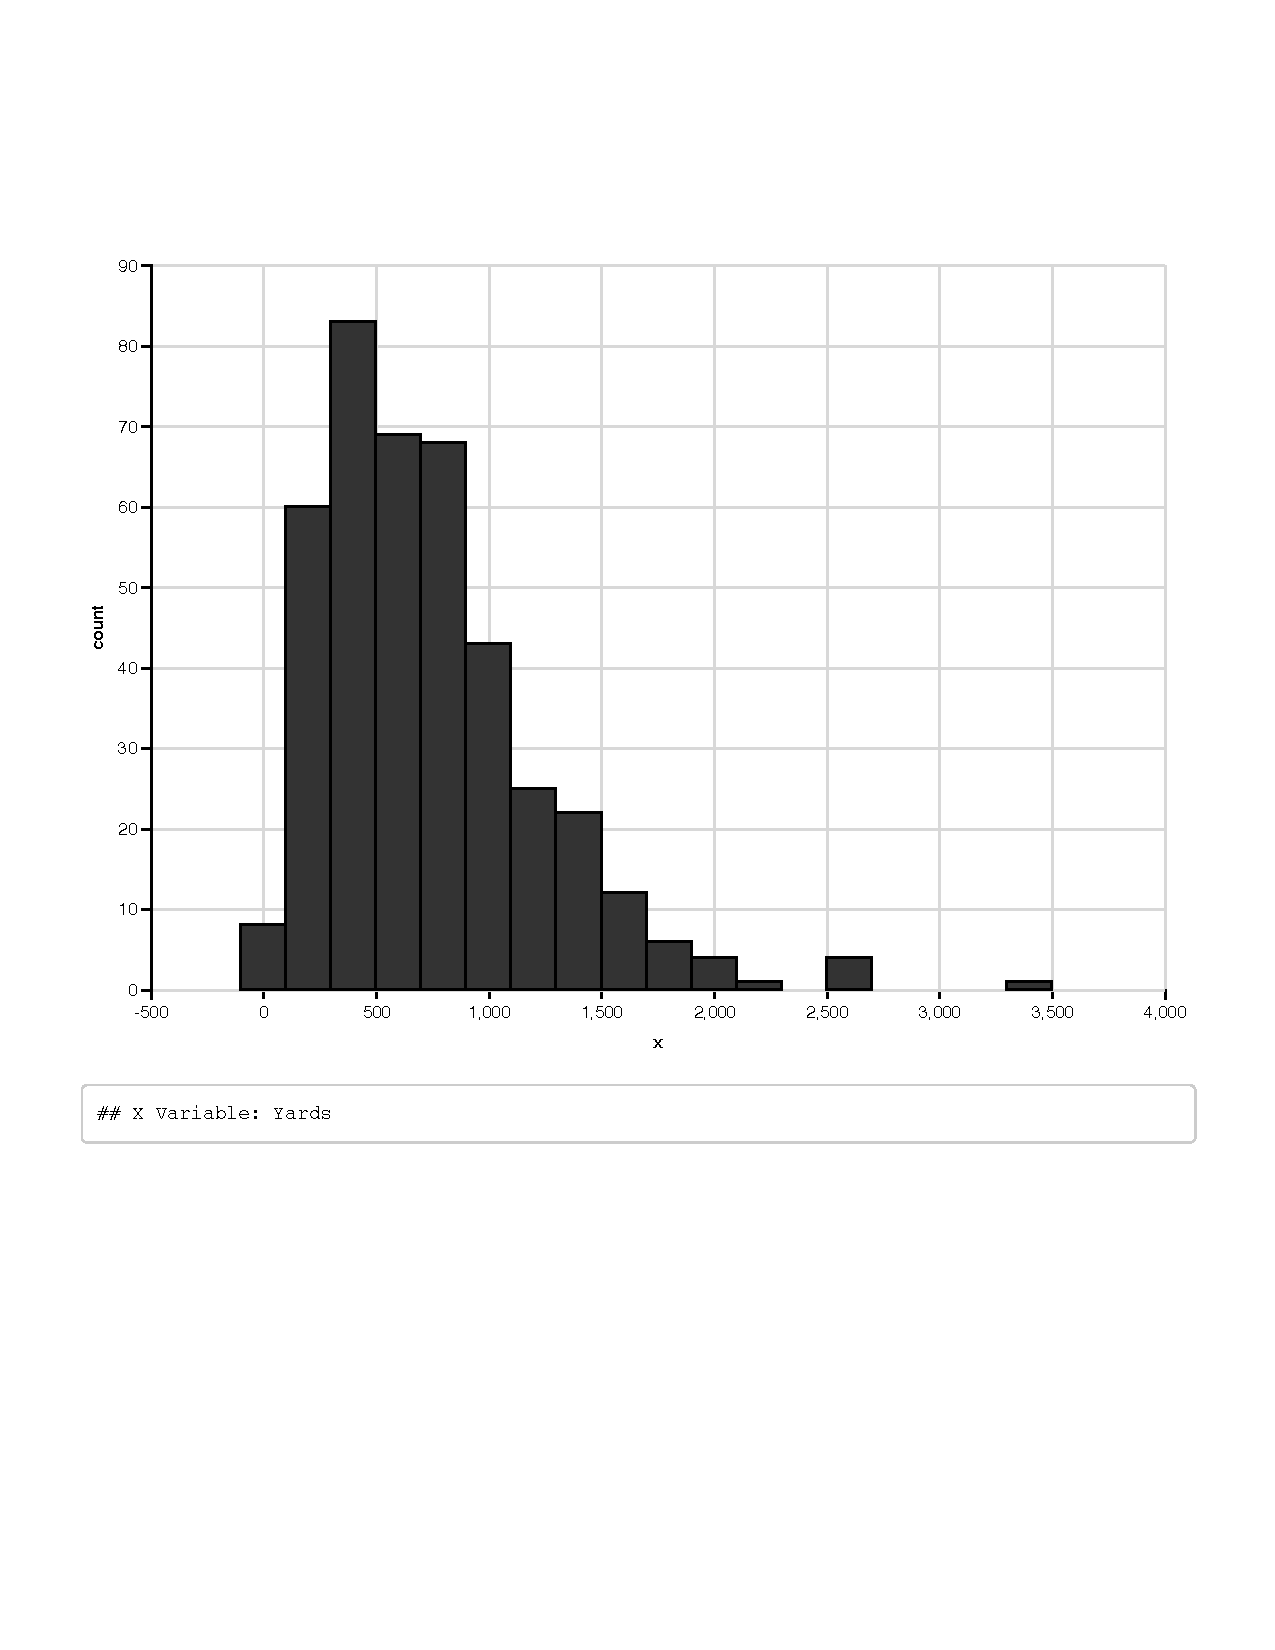
\includegraphics[width=4in]{hwk3-intRo1.pdf}

{\em The distribution is right-skewed, unimodal, centered at around 500-600 yards, with a few outliers at 2500 and 3500 yards.}

\item {\em (2 pts)} Give the five number summary for this variable.\\

{\em 29, 366, 663.5, 958.5, 3396}

\item {\em (2 pts)} Calculate the range and IQR for this variable.\\

{\em Range=3396-29=3367, IQR=592.5.}

\item {\em (2 pts)} What percentage of the quarterbacks  threw less than 366 yards? \\

{\em  25\%, 366 is $Q_1$.}

\item {\em (2 pts)} What percentage of the quarterbacks  threw more than 3396 yards?  \\

{\em 0\%, None}

\item {\em (2 pts)}Give the mean and standard deviation for this variable.\\

{\em $\bar{y}=735.0, s=482.5$} 

\item {\em (3 pts)} Explain why there is a difference of approximately 70 yards in the mean and median for this variable.\\

{\em The mean is larger than the median because the distribution is right-skewed, and outliers with large values.}

\item {\em (2 pts)} Which numerical summaries are the most appropriate for this distribution - the 5-number summary or the mean and standard deviation?  Explain your answer.

\hspace{1in} {\em 5-number summary}  \\

{\em Because the data is not symmetric and unimodal, the mean and standard deviation do not give a good summary of the center and spread of the numbers. }\\

\item {\em (3 pts)} Explore transformations of this variable to make it more symmetric. Which is best of the choices below:

\hspace{1in} {\em 0.5, because the other two make the distribution left-skewed.} 

Print a histogram of your transformed data. Compute what the transformed value of 3000 yards would be. 

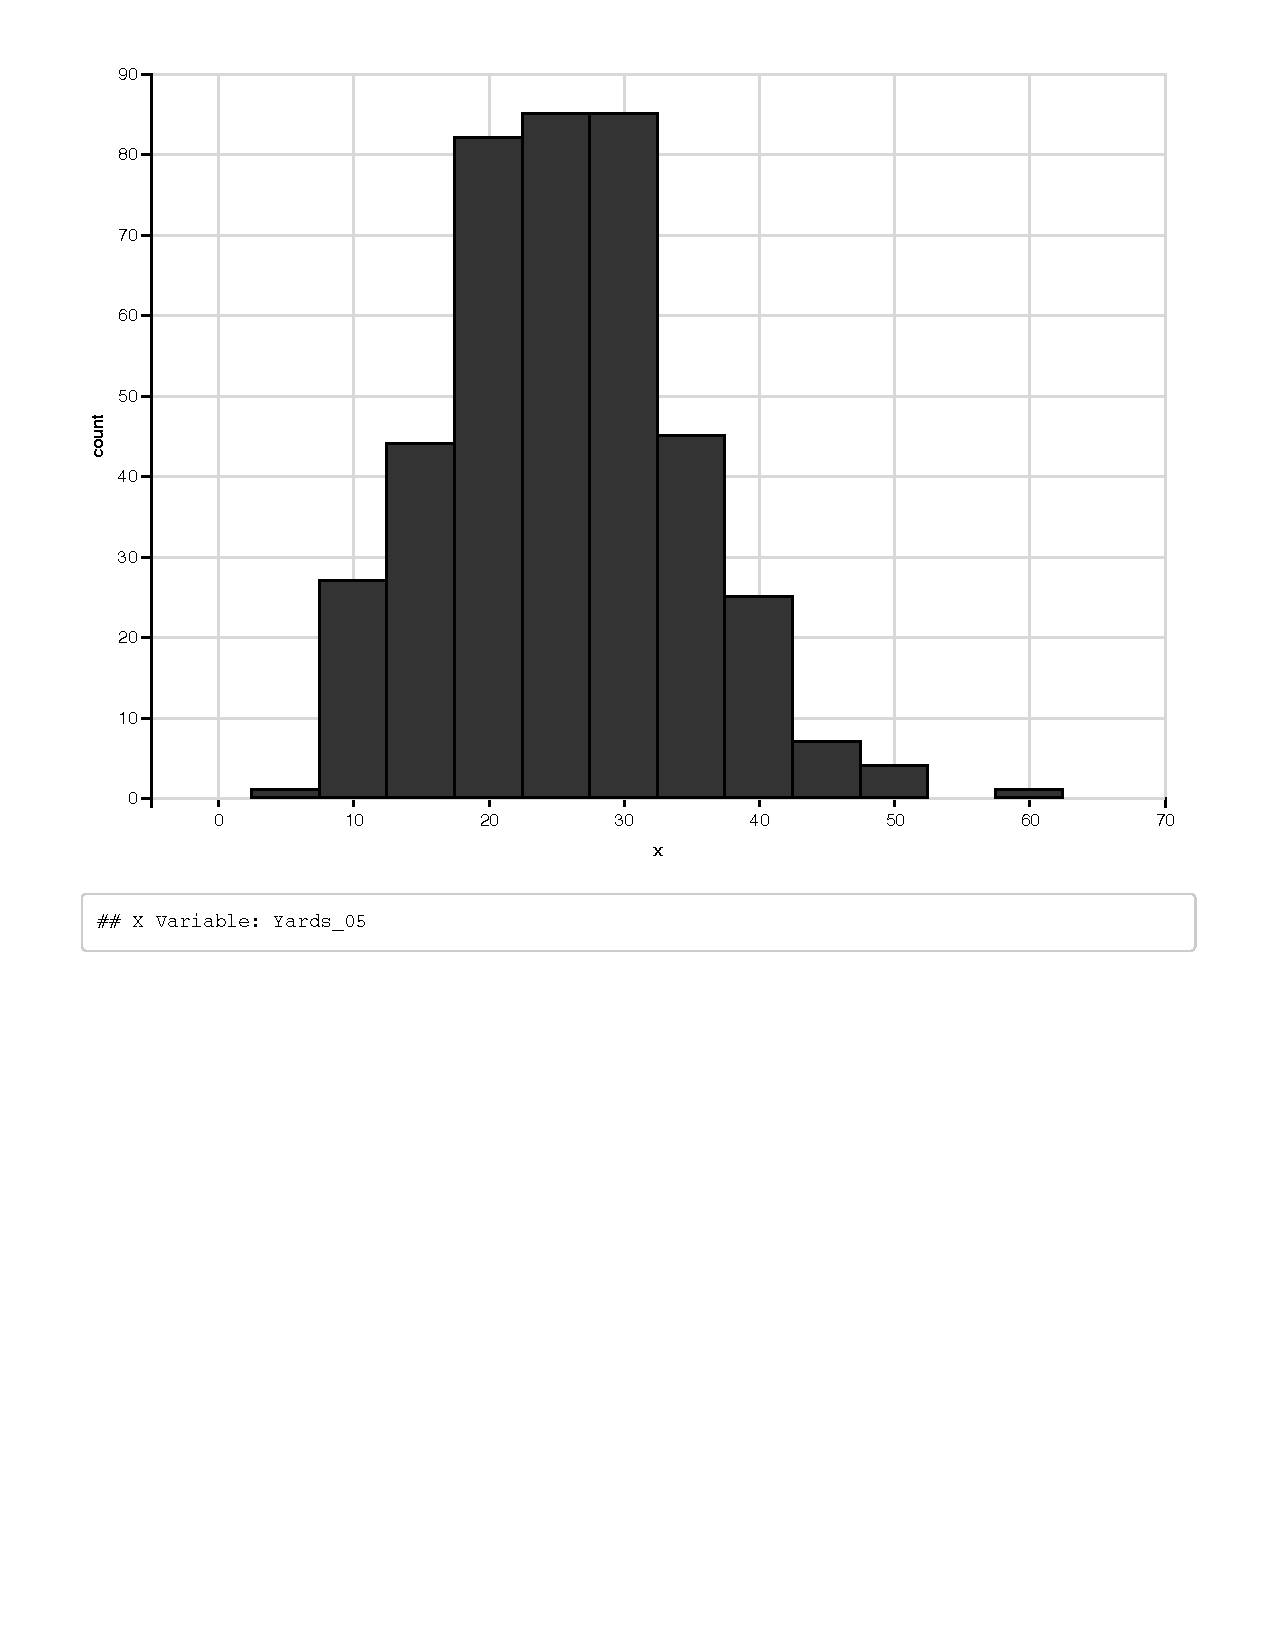
\includegraphics[width=4in]{hwk3-intRo2.pdf}

{\em There is still one outlier after the transformation. This is Blake Gimbel, who was the quarterback for Marshalltown and was widely celebrated in the news as being the bets quarterback in the state. These numbers would suggest that it is a valid praise. Although, if we also considered pass success and touchdowns some other quarterbacks have better statistics.}

{\em $\sqrt{3000} = 54.8$}

\end{enumerate}

\end{enumerate}

\end{document}
